\newcommand{\edges}{\iskey{edges}}
\newcommand{\pip}{\iskey{point-in-polygon}}
\newcommand{\lost}{\emph{line-of-sight} test}
\newcommand{\pipt}{\emph{point-in-polygon} test}

(This chapter was written by Konstantin Malakhanov. Names and addresses
of contributors to the code are found in the source code file polygon.c)

% \section{Using polylines with gstat}
% \label{sec:Using-polylines-with}
Often during interpolation one has to take into account boundaries
(edges) between data and/or interpolation points. These boundaries
can be natural, like rivers or geological faults, or man-made, like
legal boundaries. The boundaries should be used at the selection of
candidate data points, so only appropriate ones will be used for
estimation. 

For open boundaries, selected data points and the estimation point
have to be at the same side of each boundary. For closed boundaries,
data points and the estimation point all have to be either inside or
outside of each boundary.

\begin{figure}[htbp]
  \centering

  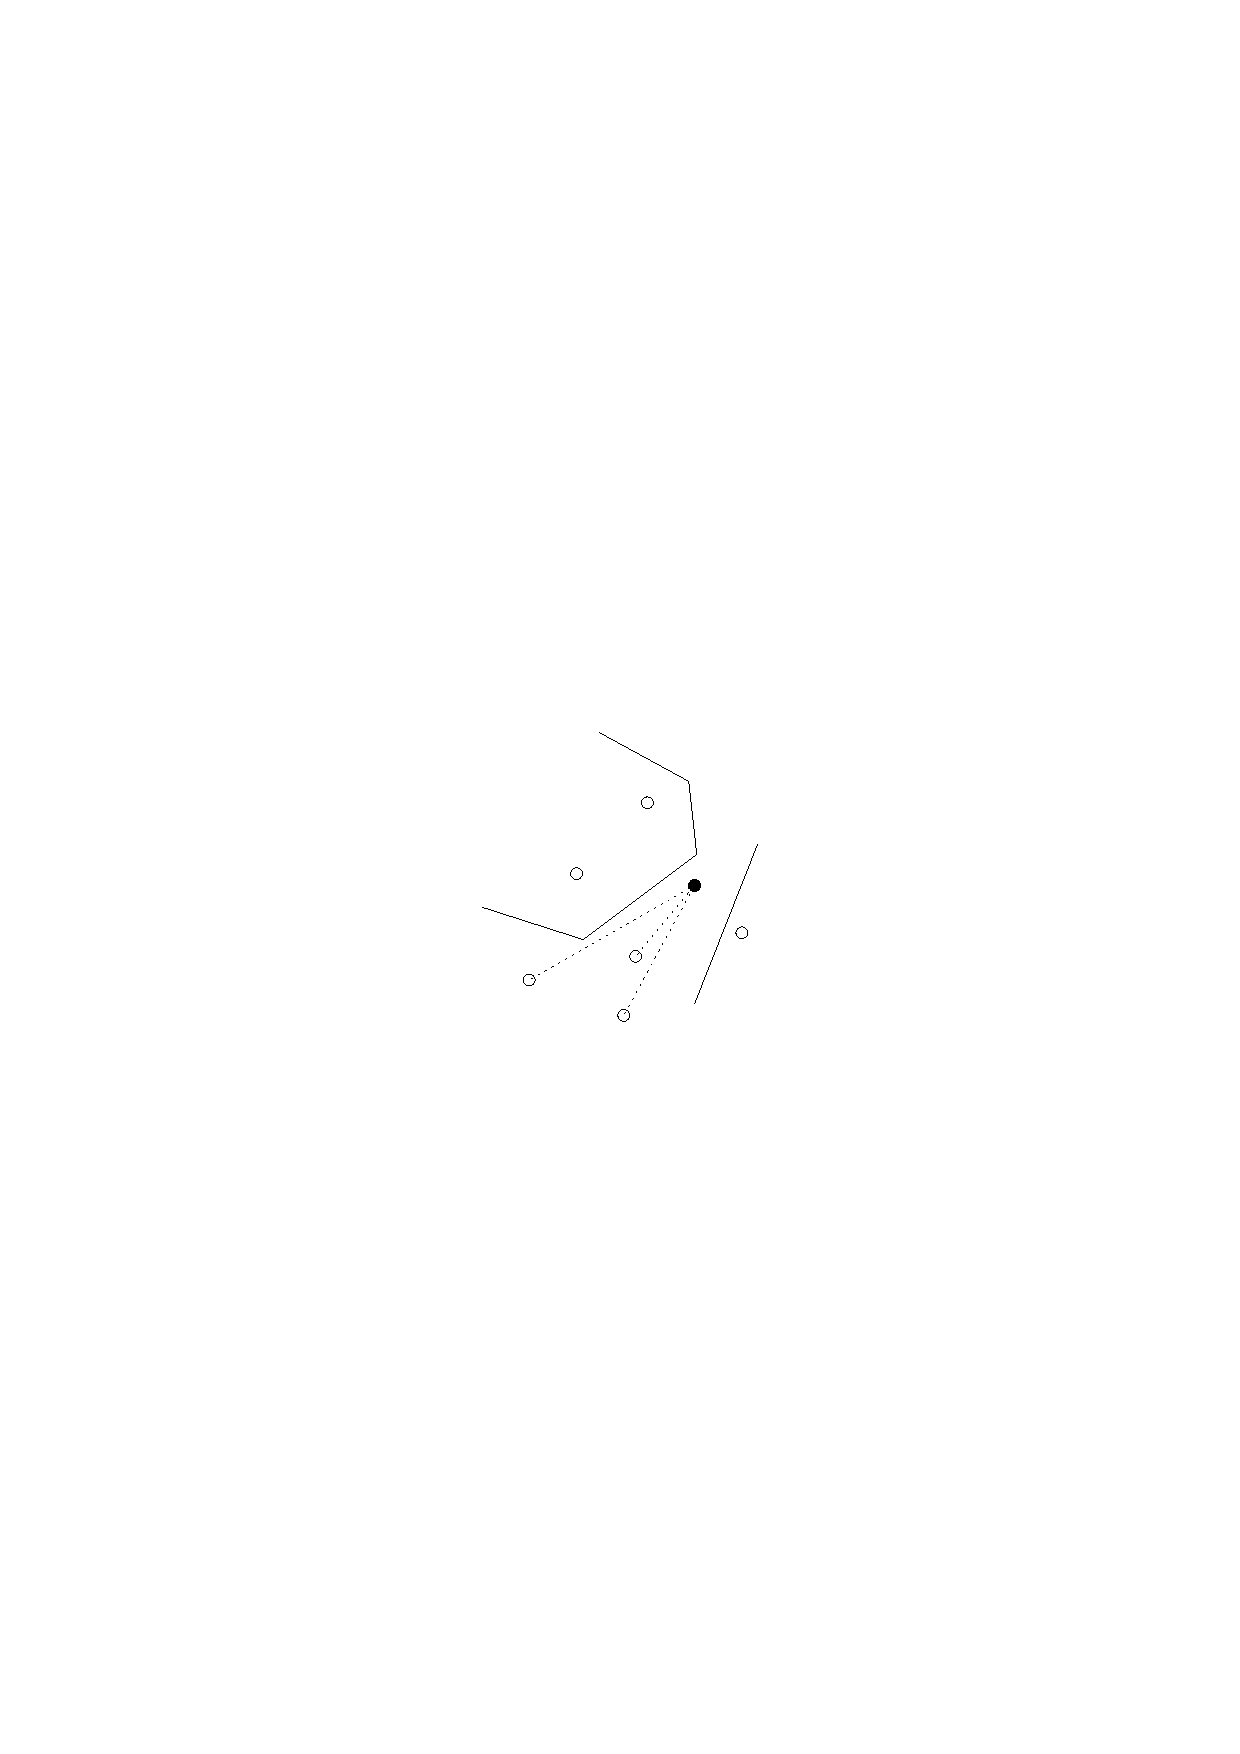
\includegraphics{\ext/open}\hspace{0.5in}%
  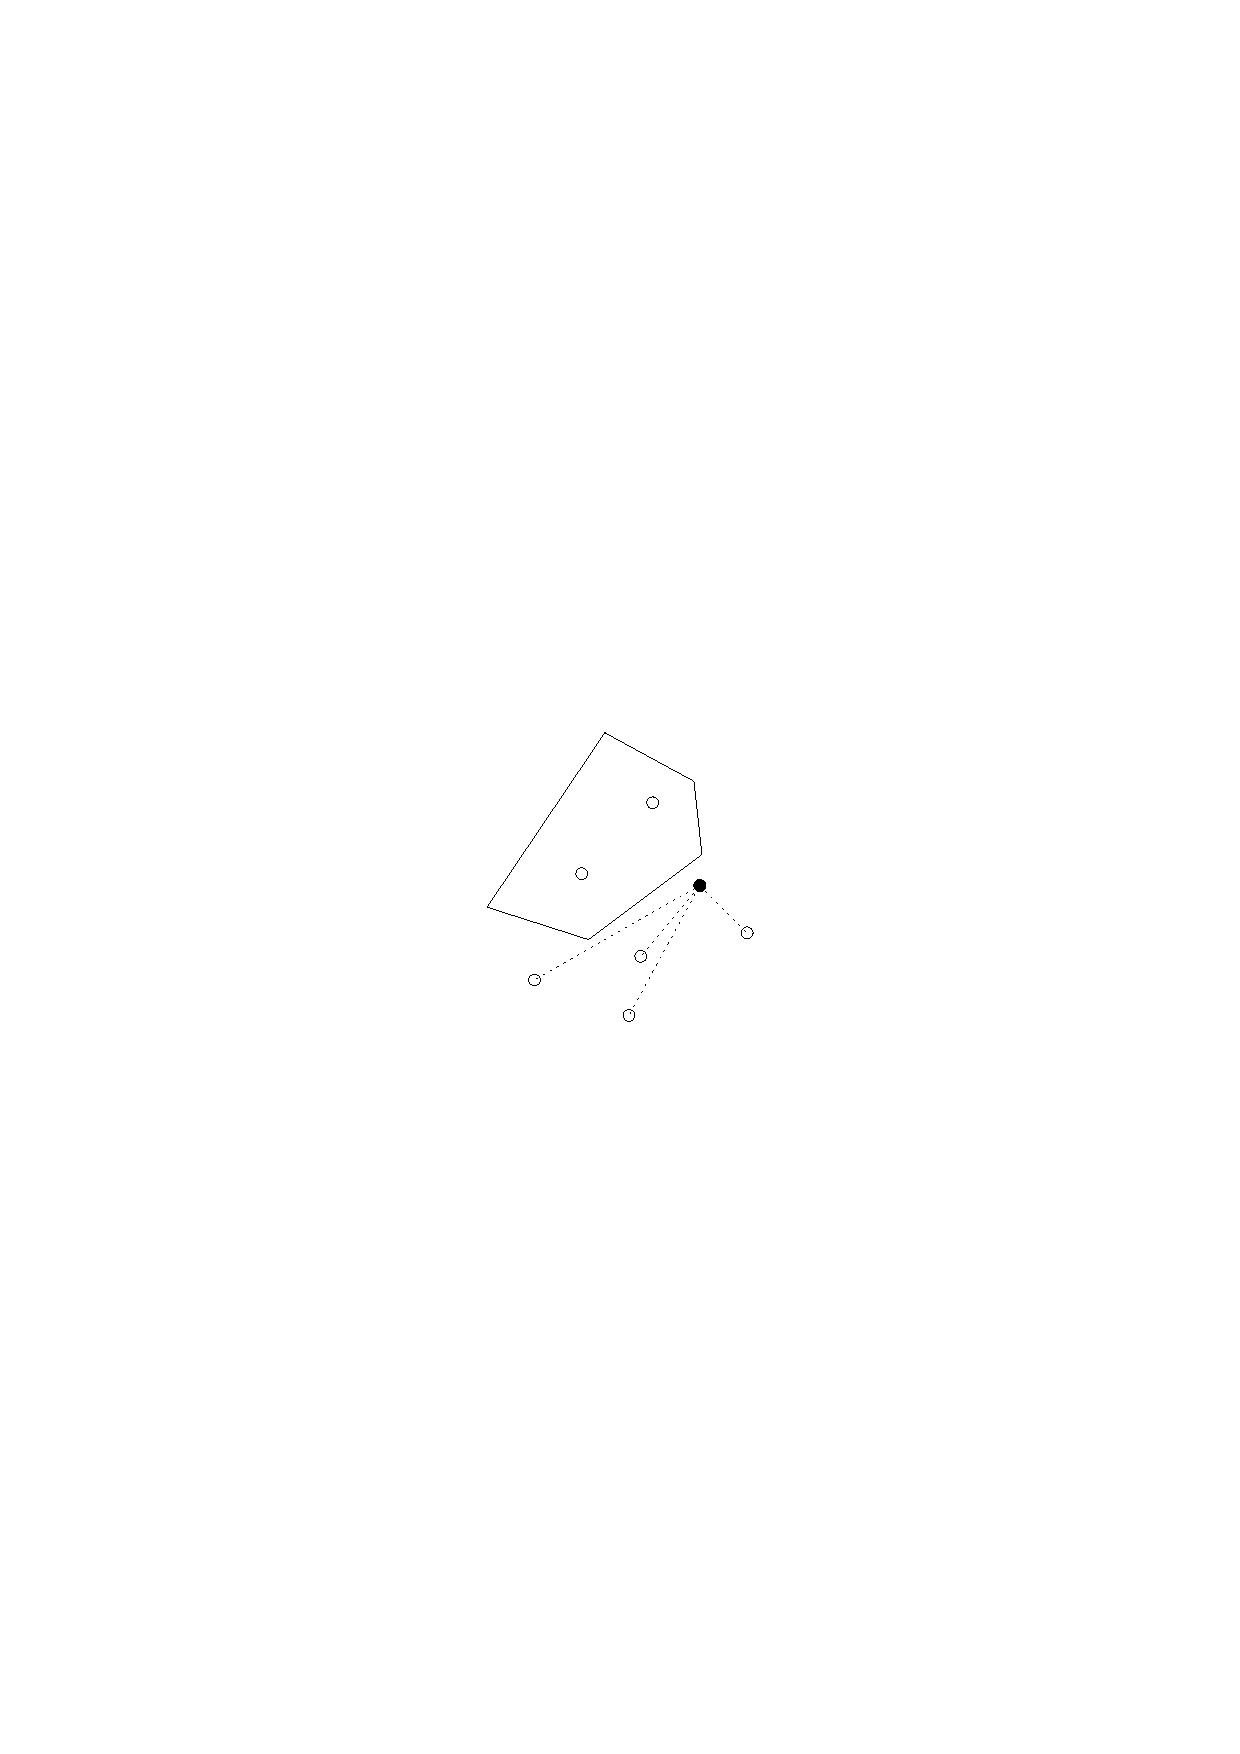
\includegraphics{\ext/closed}%    
  \caption[Most familiar cases of open and closed boundaries]%
  {Most often cases of open and closed boundaries (\textbullet~
    estimation point, $\circ$~data point). Selected data
    points are connected.}
  \label{fig:openclose}
\end{figure}

Certainly one can imagine cases of more complicated topology, with
open and closed boundaries mixed, or with connected boundaries etc. To
see an example how boundaries can be used in estimation process, see
\cite{joyce97:edges}. For general computational geometry questions,
see a book of O'Rourke \cite{rourke:compgeom} (with software available
at \url{http://cs.smith.edu/~orourke/books/ftp.html}) and
Computational Geometry FAQ \cite{faq:cg}.

To handle the ``interpolation with boundaries'' in gstat, a new
keyword (\edges{}) and a new method (\pip{}) are introduced. \edges{}
allows to take boundaries into account during estimation. \pip{}
calculates which data points are inside of given polygons.  The
\pipt{} is useful, if you want to exclude some data points outside of
given boundaries.



\section{Implementation aspects}
\label{sec:Impl-aspects}

First we introduce the following definitions:
\begin{description}
\item[polyline]  - a line of multiple connected straight segments,
\item[polygon] - a closed polyline (first and last coordinate of
 the polyline are equal).
\end{description}

For testing if two points are at the same side of a given boundary, we
use the \lost{} (fig.~\ref{fig:los}).

\begin{figure}[htbp]
  \centering
  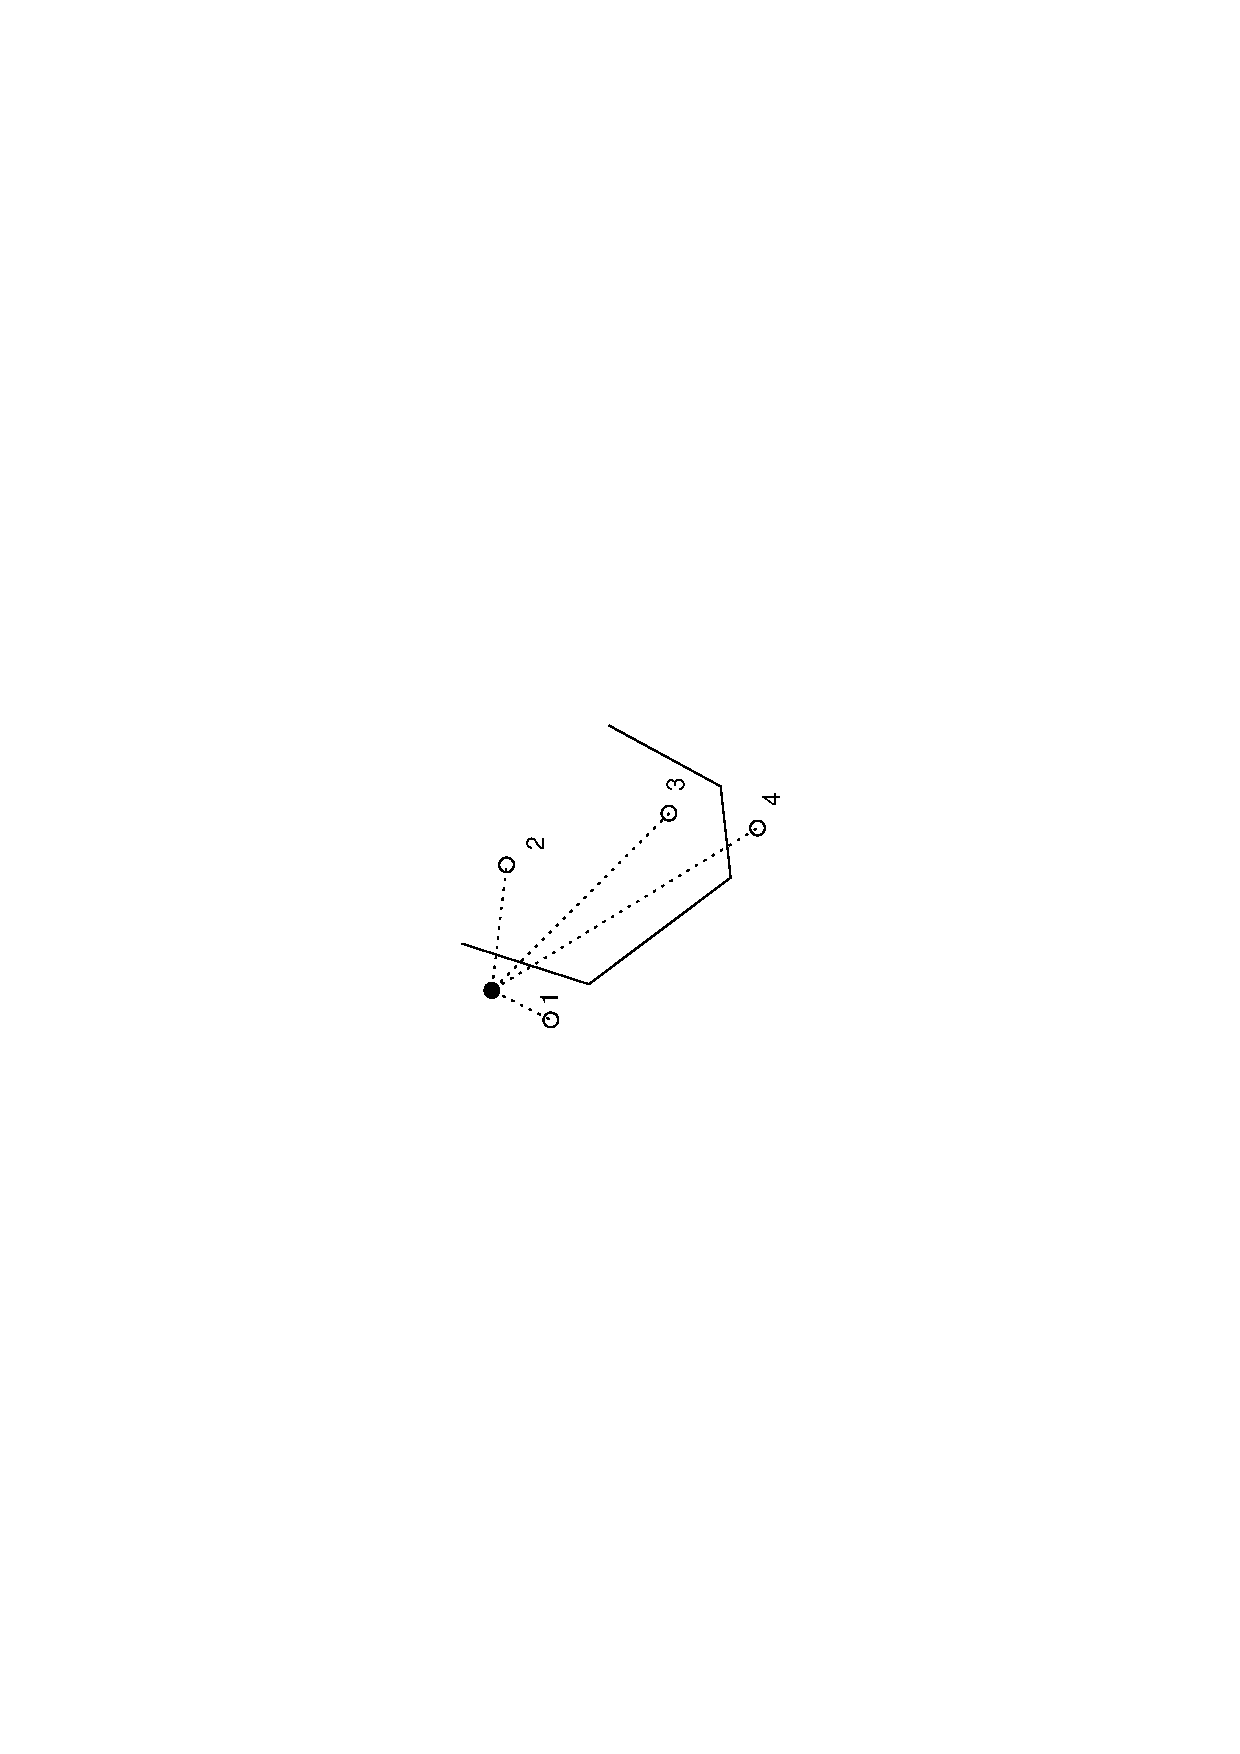
\includegraphics{\ext/los}
  \caption{Line-of-sight test}
  \label{fig:los}
\end{figure}

An (imaginary) segment goes from the estimation point to each data
point in question. If the number of segment intersections is even,
then both points are supposed to be at the same side of the boundary,
if the number of intersections is odd, they are separated by the
boundary.

In this example, the line \textbullet-1 has 0 intersections with the
edge, the lines \textbullet-2 and \textbullet-3 have only one
intersection and the line \textbullet-4 has two intersections with the
edge. So the data points 1 and 4 are assumed to be at the same side of
the edge as the estimation point.

There are some special cases in the test, like:
\begin{enumerate}
\item an estimation point or a data point lies on the edge
\item the segment goes exactly through a vertex of the edge (fig.~\ref{fig:spec_los})
  \begin{figure}[htbp]
    \centering
    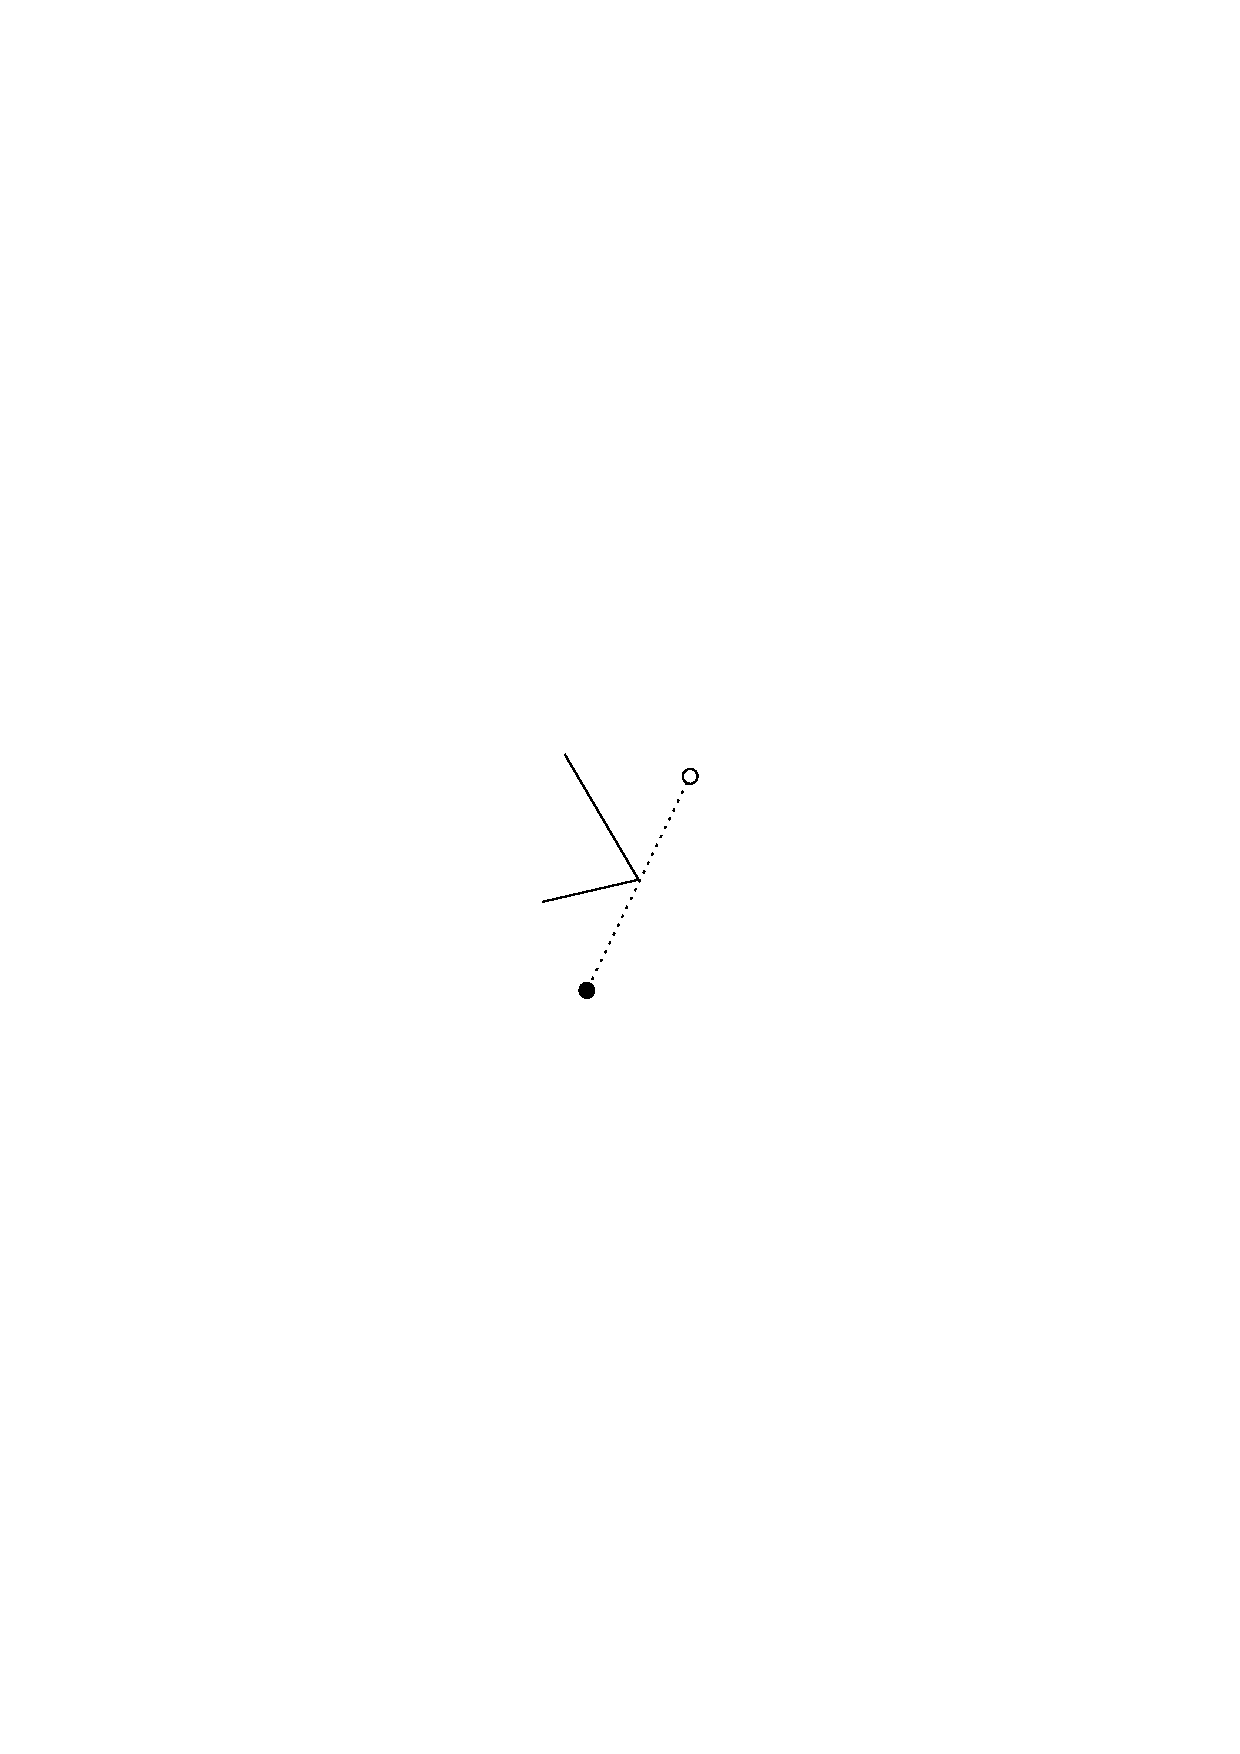
\includegraphics{\ext/spec_los}
    \caption{Special case:  the segment goes exactly through a vertex of the edge}
    \label{fig:spec_los}
  \end{figure}
\end{enumerate}

In the first case, the edge is completely ignored. In the second case,
the intersection of the segment does not count and testing will be
continued.

The results of the test depend heavily on the topological connectivity
of edges (cf.  fig.~\ref{fig:difflos}).

\begin{figure}[htbp]
  \centering
  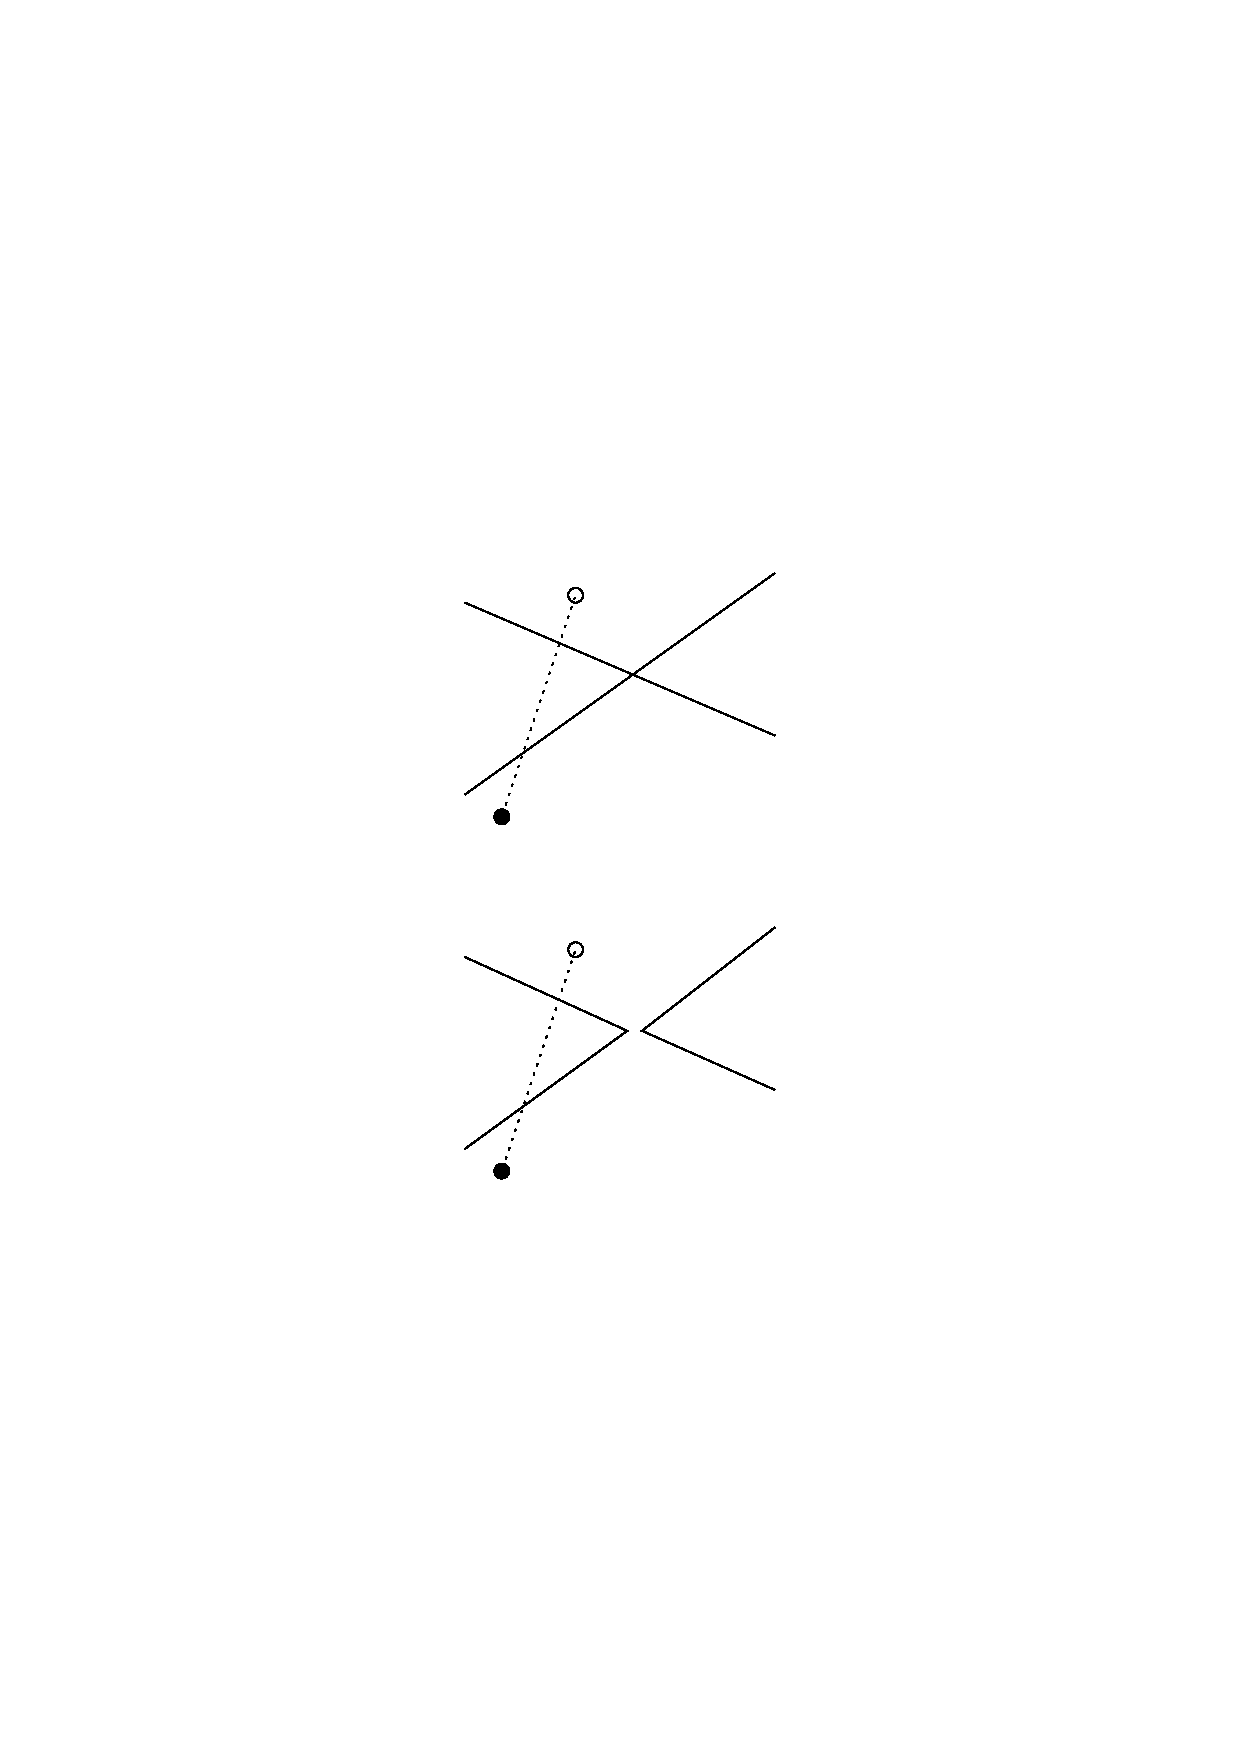
\includegraphics{\ext/difflos}
  \caption{Different results of line-of-sight test}
  \label{fig:difflos}
\end{figure}

Here at the left subfigure (boundaries are slightly shifted for better
overview) both points are connected, whereas in the right subfigure,
the points are disconnected by both line segments.

The \lost{} does not work for more complicated cases, for instance in
case of spiral boundaries (fig.~\ref{fig:badlos}).
\begin{figure}[htbp]
  \centering
  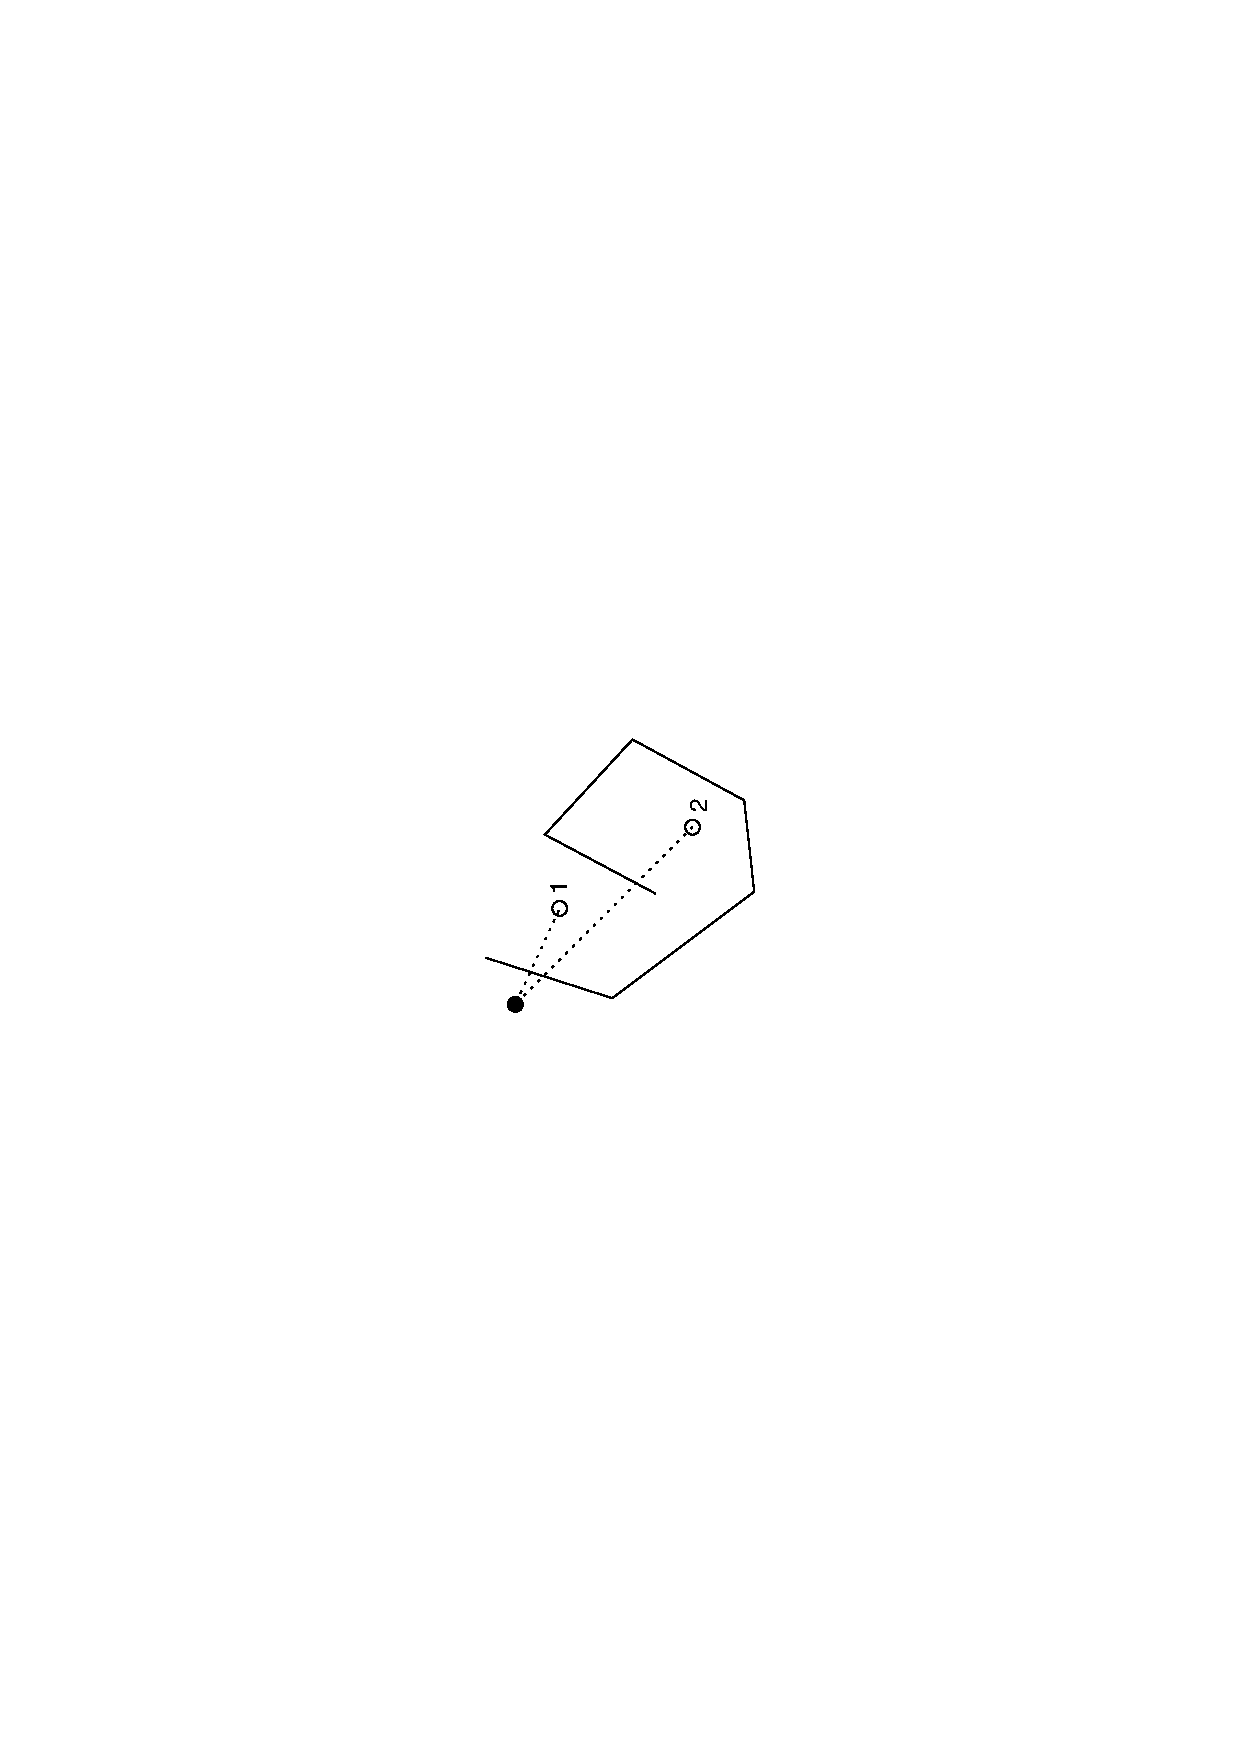
\includegraphics{\ext/badlos}
  \caption{Line-of-sight test does not work in case of spiral edges}
  \label{fig:badlos}
\end{figure}

Here the \lost{} gives wrong results. Point 1 is actually at the same
side as the estimation point and point 2 is at another side.

Concerning the question of finding the shortest path between two
points (see section \ref{sec:Vari-calc}), we are looking for the
complete solution of this problem. For now, the \lost{} should
sufficiently work in most of the usual cases.

For \pipt{} of points we have used the InPoly routine,
which is a part of the code in  \cite{rourke:compgeom}.

\begin{quote}
  InPoly test is written by Joseph O'Rourke, contributions by Min Xu,
  June 1997.
\end{quote}

For a given point it can define, if the point
\begin{itemize}
\item lies strictly inside or outside of a polygon,
\item is a vertex of a polygon,
\item lies exactly at the edge between vertexes.
\end{itemize}

\section{Formats available for input}
\label{sec:Form-avail-input}

Boundaries can be read in two formats:
\begin{description}
\item[E00 format] -- this is supposed to be ASCII ARC/INFO coverage
  format. As this format is not officially documented by ESRI, no
  warranty can be given.

  First and second lines of a file are:
\begin{verbatim*}
EXP    Name_of_coverage
ARC
\end{verbatim*}
  
  Then every polyline (polygon) has the header

\begin{verbatim}
I_ok dummy_I dummy_I dummy_I dummy_I dummy_I I_np
\end{verbatim}
  
  x-y coordinates follow then, with either one coordinate (two
  numbers) or two coordinates (four numbers) per line. \texttt{I\_np}
  is a number of coordinates in that polyline. A polyline/polygon will
  be read in, if \texttt{I\_ok} $>0$.

  
\item[``plot'' format] -- only polylines/polygons data without header.
  
  For every polyline/polygon, the first line gives a number of points.
  x-y coordinates follow then, with either one coordinate (two
  numbers) or two coordinates (four numbers) in each line.

\end{description}


%For both formats, coordinates are given in free format (white-space
%separated, possibly with e or E exponent part).

Coverage format is automatically recognized by \texttt{EXP} as the
first word of a file.

\section{New keywords}
\label{sec:New-keywords}

\begin{enumerate}
\item \edges{}. To use like:
  
\begin{verbatim}
  edges: "file1","file2",...;
\end{verbatim}  
  Given boundary files will be read in and the boundaries will be used
  during neighborhood search. You can give both polylines and polygons.
  
\item \pip{}. To use like: 
  
\begin{verbatim}
  method: point-in-polygon;
\end{verbatim}  
  With given point locations (through \texttt{data} statement), gstat
  will search which polygons the points are in.  The output is a list
  of locations with a file number in the prediction column and a
  polygon number in the variance column of the output file. For points
  inside a polygon, this will be numbers counting  from 0.  Locations
  which are not inside of any polygon will have NA in both columns.
  
\end{enumerate}   


\section{Using \pipt{}}
\label{sec:Using-pipt}

To use \pipt{}, give through data statement the locations of points you
want to test for being inside of given \edges{}.

For this test, polylines do not have to be closed -- they are treated
as closed anyway. Points on the polyline or coincident with vertices
are assumed to be inside of the polygon.

A data point gets the number of the first of given polygons it is in,
or NA otherwise. You can parse the output with tools you have at the
hand (grep, awk, Perl\dots{}) and select points you are interested in.

\section{Using polylines with interpolation}
\label{sec:int-poly}


Edges are used for neighborhood selection after testing for
radius/maximum number of data points. The global selection will be
changed as well.

Suppose we have an estimation point (to get an interpolated/simulated
value at) and a data point. First, all relevant edges in the search
neighborhood are found. This works by comparing the bounding boxes of
all edges with the box region of the estimation point (fig.~\ref{fig:boxtest}).

\begin{figure}[htbp]
  \centering
  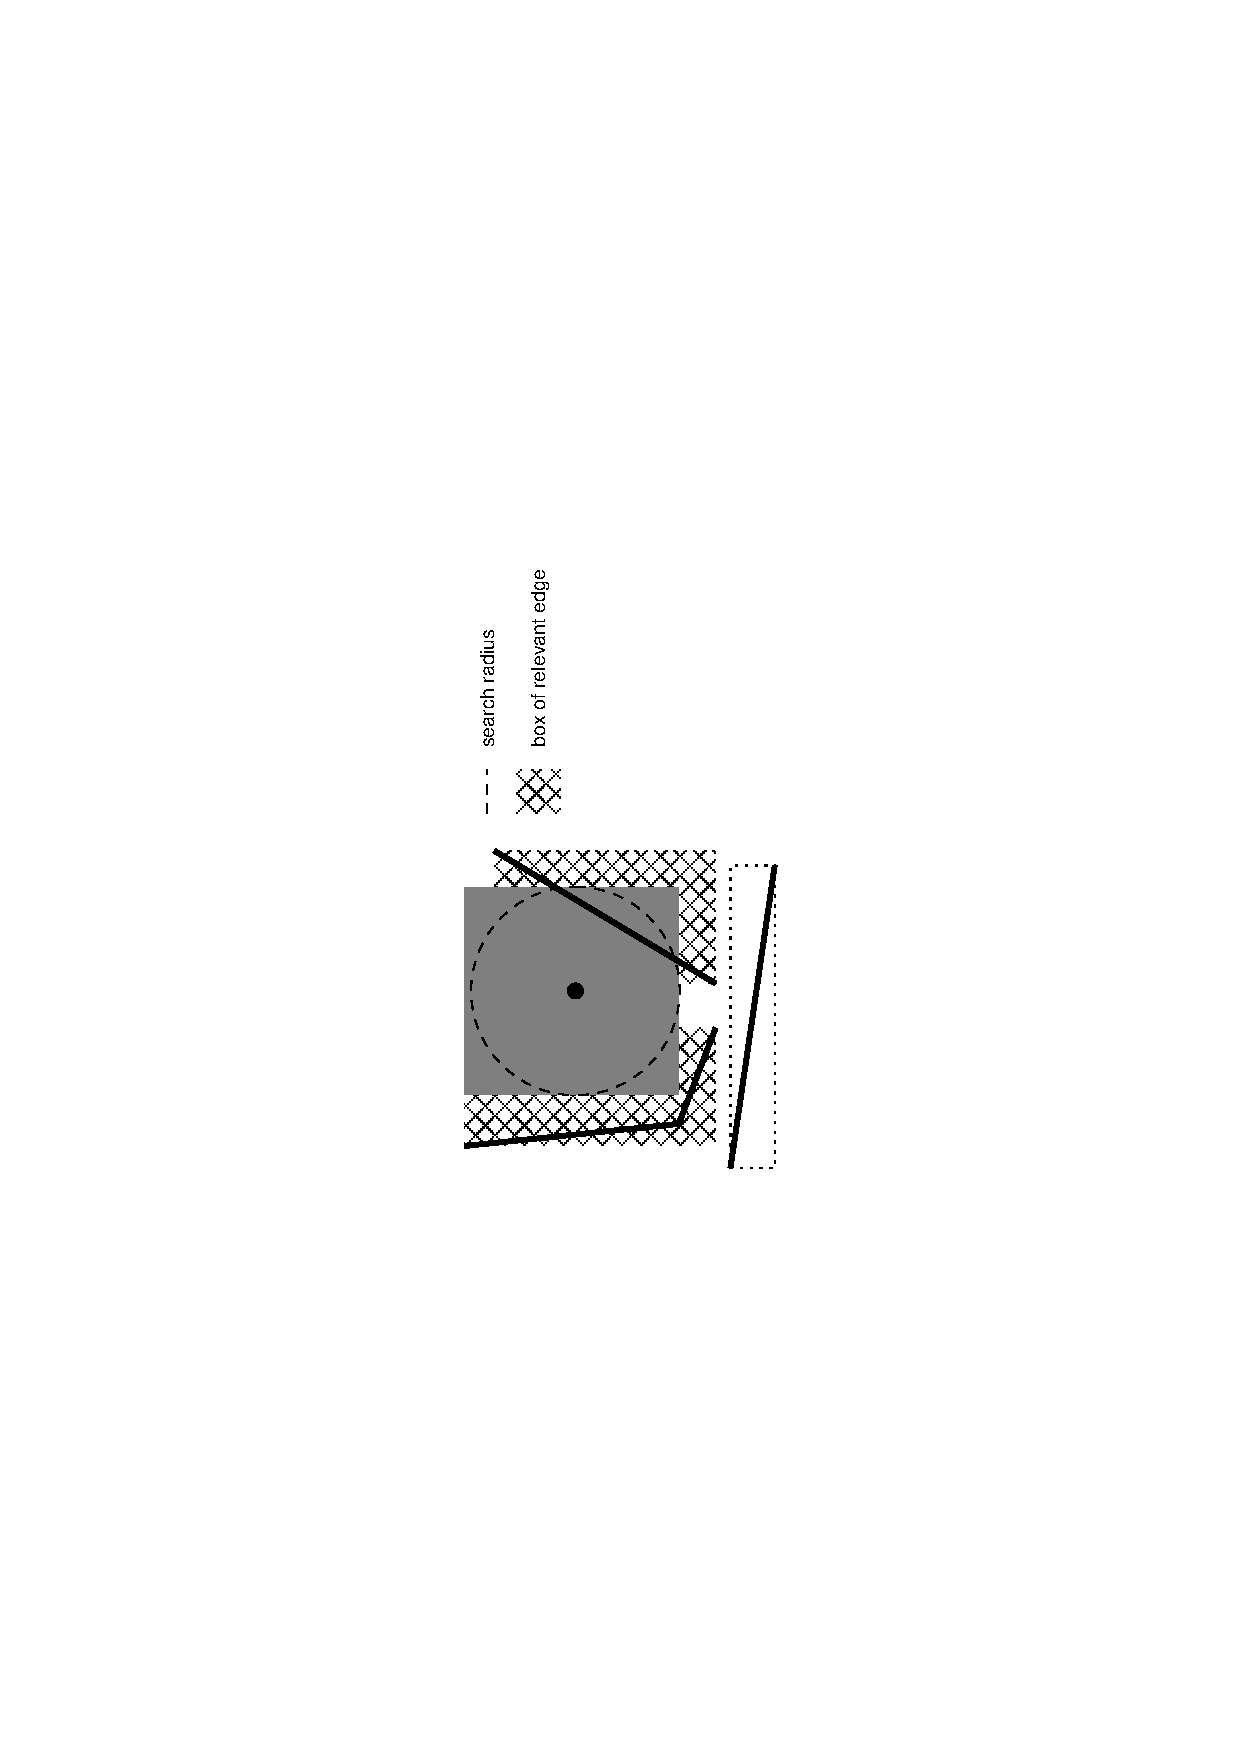
\includegraphics{\ext/boxtest}
  \caption{Test of edges' extents}
  \label{fig:boxtest}
\end{figure}

                                %If the estimation point lies directly at any closed polyline, this
                                %polyline is ignored.

Then, depending on the type of the polyline (open/closed), the \lost{}
or the \pipt{}  is performed for the estimation point and all data
points found so far.


During the testing, if the estimation point is found being on any
edge, this edge is skipped for further testing for this estimation
point for all data points. If a data point lies on any edge, this edge
will not be tested for this data point anymore.

The edges test is repeated for all edges found. A data point will be
used, if it passes the test for all edges.

As you can see, all testing is done by brute-force testing. So if you
have a lot of edges, with all of them relevant for most of the data
points, this will slow down interpolation/simulation a lot. Smarter
edges searching is for sure possible, for example, using line
quadtrees.  Better testing can probably be implemented in
connection with finding the shortest path between two points.



\section{Distance calculation with boundaries}
\label{sec:Vari-calc}

Both variogram calculation and interpolation depend on the
calculation of distance between two points. Without edges, this
distance is simply an Euclidean one. Taking edges into account, the
situation will be more difficult (fig.~\ref{fig:indirect}).

\begin{figure}[htbp]
  \centering
  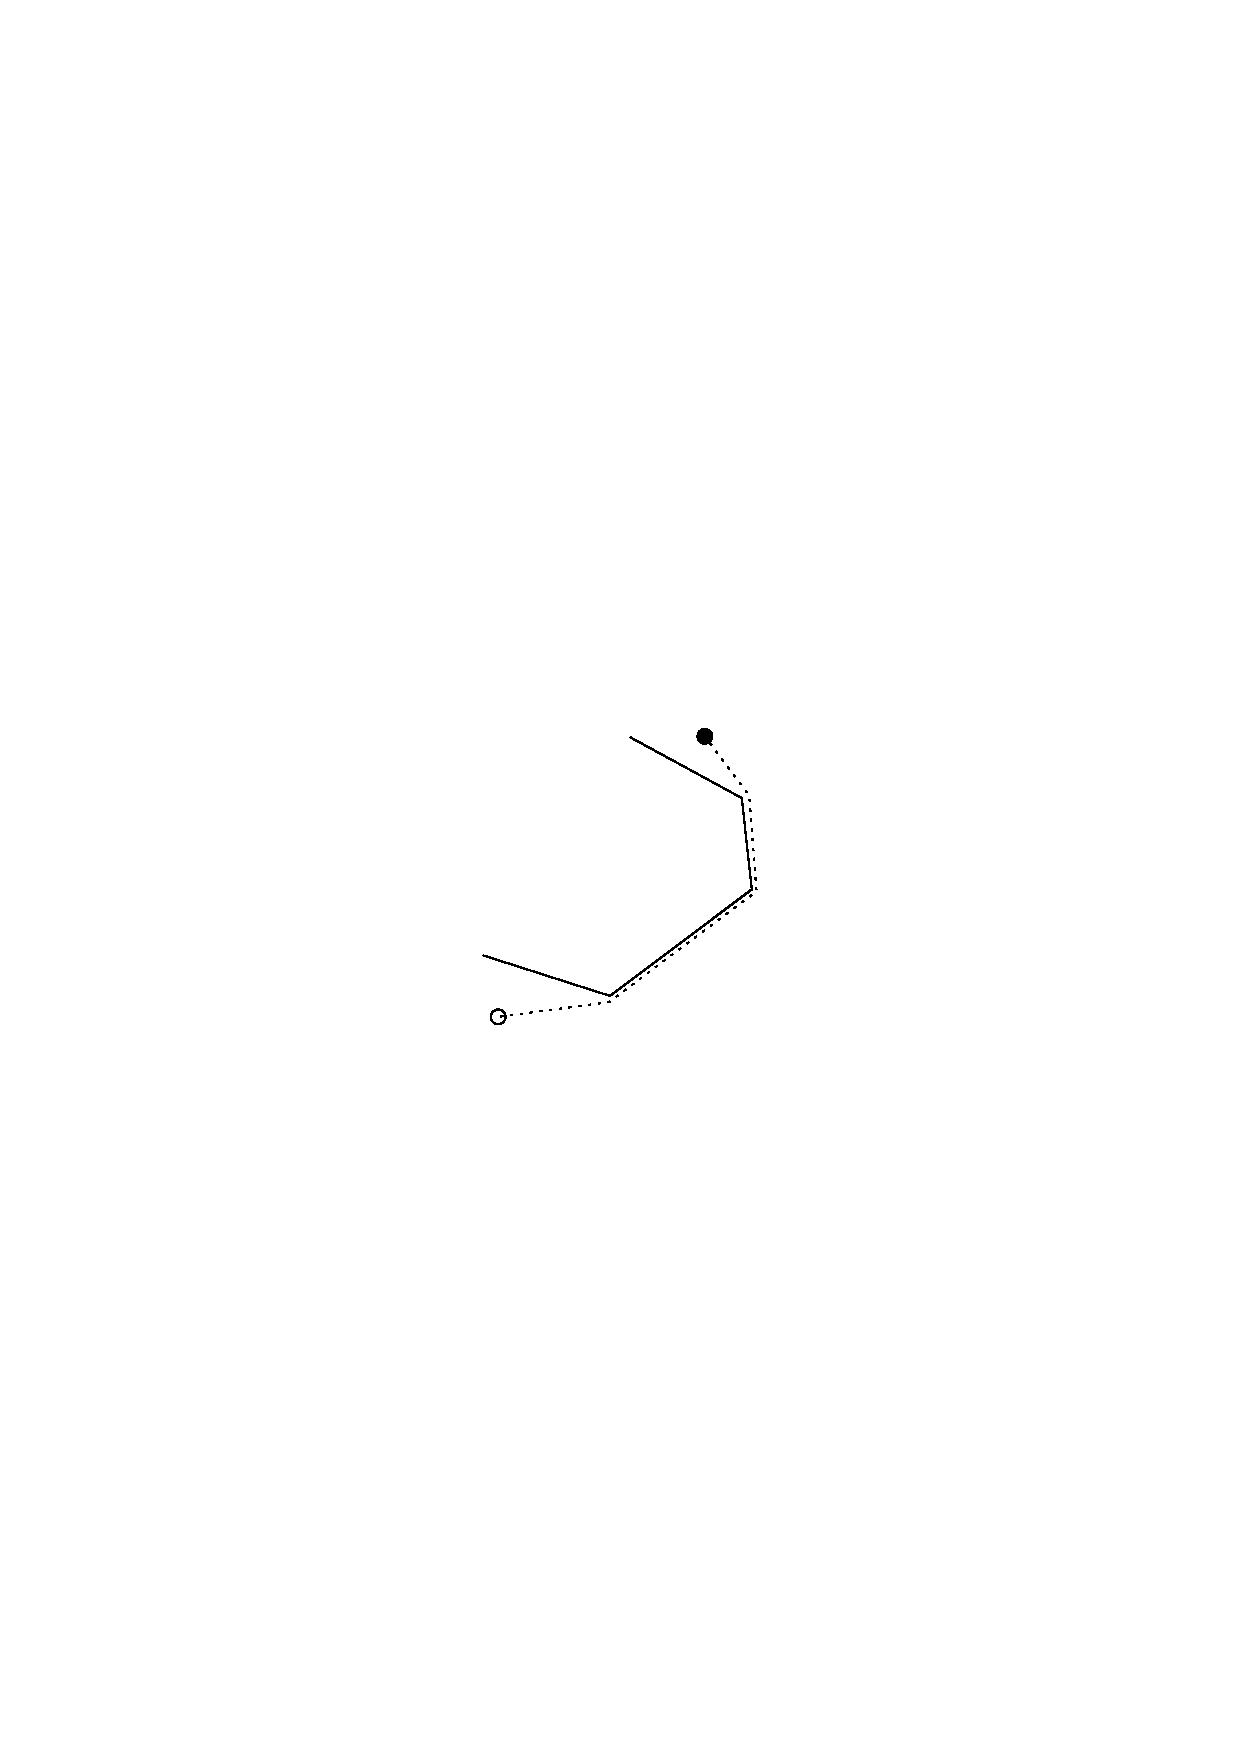
\includegraphics{\ext/dist}
  \caption{Indirect path between two points}
  \label{fig:indirect}
\end{figure}

Depending on the boundary topology, a shortest path could be not so
obvious at all.

There is a well-known solution for the problem of finding the shortest
path between points separated by some polygons (i.e. building the
connection graph and using Dijkstra's algorithm). We were not able to
find any ready solution for the case of \emph{open} polylines. So
until the solution is found, the distance between two points will be
calculated without taking boundaries into account. We suppose that the
correct solution will also eliminate the problems of the \lost.
